%%%%%%%%%%%%%%%%%%%%%%%%%%%%%%%%%%%%%%%%%%%%%%%%%%%%%%%%%%%%%%%%%%%%%%%%%%%%%%

\documentclass{l3deliverable}

%%%%%%%%%%%%%%%%%%%%%%%%%%%%%%%%%%%%%%%%%%%%%%%%%%%%%%%%%%%%%%%%%%%%%%%%%%%%%%

\usepackage{graphicx}%
%
%\usepackage{svn-multi}%
%\svnid{$Id: d3.tex 2500 2011-09-21 15:56:43Z tws $}

%\version{SVN Revision \svnrev~ \

%Made \svnday/\svnmonth/\svnyear~ by \svnauthor}

\usepackage{tabularx}%
\usepackage{url}%
\usepackage{usecasedescription}%

%%%%%%%%%%%%%%%%%%%%%%%%%%%%%%%%%%%%%%%%%%%%%%%%%%%%%%%%%%%%%%%%%%%%%%%%%%%%%%
%% Check these macro values for appropriateness for your own document.

\title{Requirements Document}

\author{Author 1 \\
        Author 2 \\
        Author 3 \\
        ...}

\date{9 January 2009}

\deliverableID{D3}
\project{PSD3 Group Exercise 1}
\team{X}

%%%%%%%%%%%%%%%%%%%%%%%%%%%%%%%%%%%%%%%%%%%%%%%%%%%%%%%%%%%%%%%%%%%%%%%%%%%%%%

\begin{document}

%%%%%%%%%%%%%%%%%%%%%%%%%%%%%%%%%%%%%%%%%%%%%%%%%%%%%%%%%%%%%%%%%%%%%%%%%%%%%%

\maketitle

\tableofcontents

\newpage

%%%%%%%%%%%%%%%%%%%%%%%%%%%%%%%%%%%%%%%%%%%%%%%%%%%%%%%%%%%%%%%%%%%%%%%%%%%%%%
%% Standard section for all documents

\section{Introduction}

\subsection{Identification}

\subsection{Related Documentation}

\subsection{Purpose and Description of Document}

\subsection{Document Status and Schedule}

%%%%%%%%%%%%%%%%%%%%%%%%%%%%%%%%%%%%%%%%%%%%%%%%%%%%%%%%%%%%%%%%%%%%%%%%%%%%%%

\section{Extended Problem Defintion}

%%%%%%%%%%%%%%%%%%%%%%%%%%%%%%%%%%%%%%%%%%%%%%%%%%%%%%%%%%%%%%%%%%%%%%%%%%%%%%

Give an extended description of the problem here.

%%%%%%%%%%%%%%%%%%%%%%%%%%%%%%%%%%%%%%%%%%%%%%%%%%%%%%%%%%%%%%%%%%%%%%%%%%%%%%

\section{System Scope}

Give an overview of the system here, in the context of the surrounding
environment.  Use case diagrams can be used to illustrate the
interactions between actors in the environment and the system.

You should explain the assumptions you have made in defining the
boundary of the system (i.e. what the system will and will not do).

Describe any conflicts in requirements expressed by different
stakeholders, how you resolved them and why.

%%%%%%%%%%%%%%%%%%%%%%%%%%%%%%%%%%%%%%%%%%%%%%%%%%%%%%%%%%%%%%%%%%%%%%%%%%%%%%

\subsection{System Actors}

\section{Actors}
\label{sec:actors}

\begin{figure}[t]
  \label{fig:actors}
  \caption{Actors of the system}
  \begin{center}
    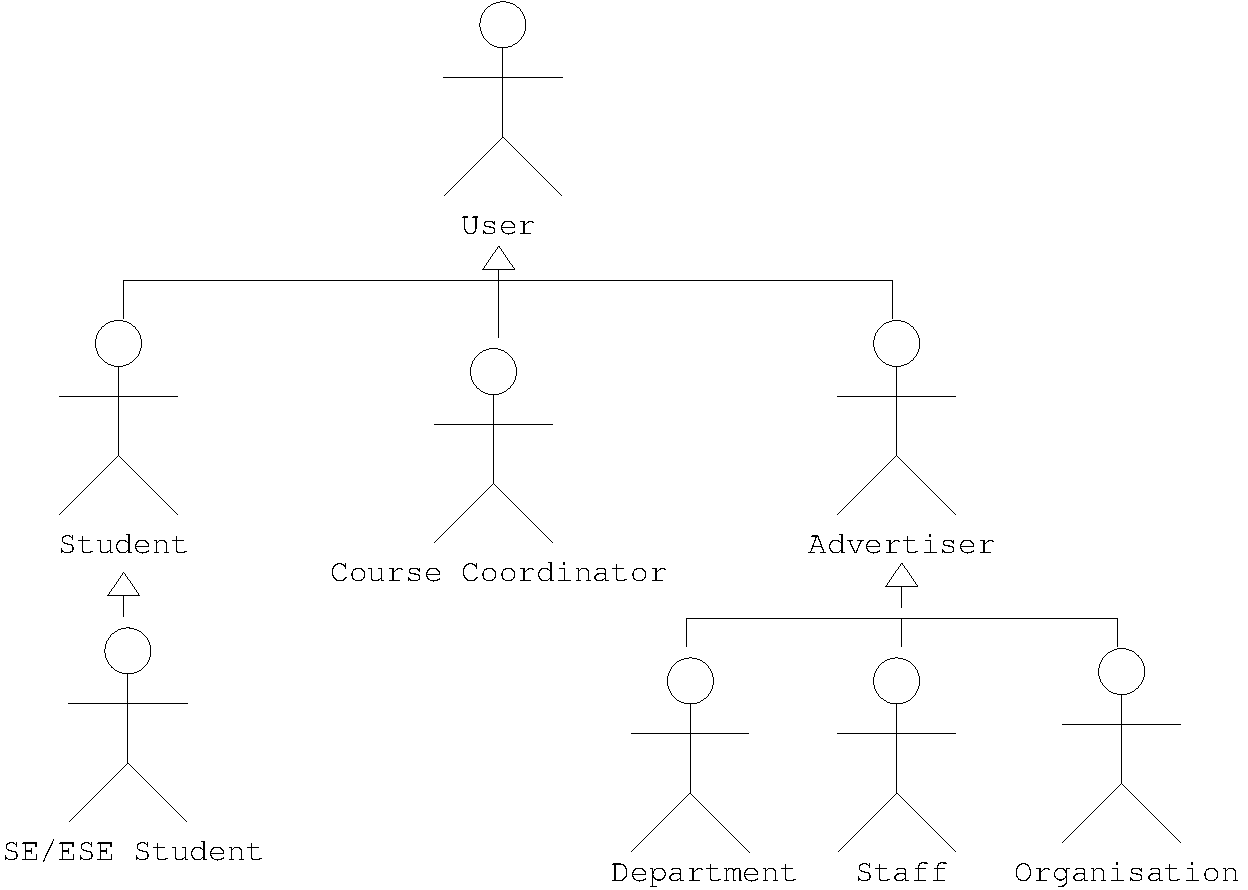
\includegraphics[width=0.9\textwidth]{img/actors.pdf}
  \end{center}
\end{figure}

Figure \ref{fig:actors} illustrates the relationships between actor roles in the system.
A short summary of the actors is given below:

\begin{description}
\item[User]{A user of the system}
\item[Advertiser] {A user who can advertise internships}
\item[Organisation] {An advertiser belonging to an organisation outwith the University}
\item[Academic] {An advertiser who is an academic at the University}
\item[Student] {A user who is a Computing Science student at the University}
\item[SE/ESE Student] {A student studying Software Engineering or Electronics and Software Engineering}
\item[Staff] {A user who is a member of staff at the University}
\item[Course Coordinator] {A type of Staff who acts as the bridge between Advertisers and Students}
\end{description}

\section{Use Cases}
\label{sec:usecases}

This section describes the required functionality for the Internship Management System as \textbf{X} groups of related use cases. 
The core use cases for the system are:

\begin{itemize}
  \item{Common Utilities (Section \textbf{X})}
    \begin{itemize}
      \item{Search for Advert}
      \item{Search for User}
      \item{\ldots}
    \end{itemize}
  \item{Submitting Advertisements (Section X)}
    \begin{itemize}
    \item{Submit advertisement for review}
    \item{Review advertisement}
    \item{Comment advertisement}
    \item{Publish advertisement}
    \end{itemize}
\end{itemize}


Give descriptions of each of the actors that you have identified as
interacting with the system.

%%%%%%%%%%%%%%%%%%%%%%%%%%%%%%%%%%%%%%%%%%%%%%%%%%%%%%%%%%%%%%%%%%%%%%%%%%%%%%

\subsection{Domain Model}

Explain the elements of the domain here.

%%%%%%%%%%%%%%%%%%%%%%%%%%%%%%%%%%%%%%%%%%%%%%%%%%%%%%%%%%%%%%%%%%%%%%%%%%%%%%

\section{Use Case Descriptions}

This is a collection of use case descriptions (one per use case).
Think carefully about how to group these descriptions in the document.
You can use the template style provided to format your descriptions:

\begin{UseCaseTemplate}
\UseCaseLabel{}
\UseCaseDescription{}
\UseCaseRationale{}
\UseCasePriority{}
\UseCaseStatus{}
\UseCaseActors{}
\UseCaseExtensions{}
\UseCaseIncludes{}
\UseCaseConditions{}
\UseCaseNonFunctionalRequirements{}
\UseCaseScenarios{}
\UseCaseRisks{}
\UseCaseUserInterface{}
\end{UseCaseTemplate}

%%%%%%%%%%%%%%%%%%%%%%%%%%%%%%%%%%%%%%%%%%%%%%%%%%%%%%%%%%%%%%%%%%%%%%%%%%%%%%

\section{Non Functional Requirements}

Describe the non-functional requirements for the system here, giving a
rationale (traceable to your requirements gathering) for each.  You
will need to think about how to group/structure requirements in this
section.

%%%%%%%%%%%%%%%%%%%%%%%%%%%%%%%%%%%%%%%%%%%%%%%%%%%%%%%%%%%%%%%%%%%%%%%%%%%%%%

\section{Summary}

Give a (very short) summary of the key aspects of the requirements
specification.

%%%%%%%%%%%%%%%%%%%%%%%%%%%%%%%%%%%%%%%%%%%%%%%%%%%%%%%%%%%%%%%%%%%%%%%%%%%%%%

\appendix

Some suggested appendices are included below.

Appendices should be used to include information not completely
necessary to the understanding of the main document.

\section{Glossary}

Definitions.

\section{Scenarios}

A collection of scenarios you developed to exercise and refine your
use cases.

\section{Stakeholder Interview Documentation}

Any evidence you gathered from stakeholders relevant to your
requirements description.  You don't need to include everything
verbatim here, but summary documents, for example, identifying the key
points you identified (particularly if they relate to requirements
conflicts) can be useful.

\section{Stakeholder Panel Documentation}

(see above)

%%%%%%%%%%%%%%%%%%%%%%%%%%%%%%%%%%%%%%%%%%%%%%%%%%%%%%%%%%%%%%%%%%%%%%%%%%%%%%

\end{document}

%%%%%%%%%%%%%%%%%%%%%%%%%%%%%%%%%%%%%%%%%%%%%%%%%%%%%%%%%%%%%%%%%%%%%%%%%%%%%%
